% ==========================================================
% ENTREGA 1 — A pergunta do trabalho
% Versão compatível: article + natbib (sem abntex2)
%
% Compilar:
%   RStudio: botão "Compile PDF" (com knitr configurado)
%   Terminal: Rscript -e "knitr::knit2pdf('entrega-1-pergunta.Rnw')"
% ==========================================================
\documentclass[12pt,a4paper,oneside]{article}\usepackage[]{graphicx}\usepackage[]{xcolor}
% maxwidth is the original width if it is less than linewidth
% otherwise use linewidth (to make sure the graphics do not exceed the margin)
\makeatletter
\def\maxwidth{ %
  \ifdim\Gin@nat@width>\linewidth
    \linewidth
  \else
    \Gin@nat@width
  \fi
}
\makeatother

\definecolor{fgcolor}{rgb}{0.345, 0.345, 0.345}
\newcommand{\hlnum}[1]{\textcolor[rgb]{0.686,0.059,0.569}{#1}}%
\newcommand{\hlsng}[1]{\textcolor[rgb]{0.192,0.494,0.8}{#1}}%
\newcommand{\hlcom}[1]{\textcolor[rgb]{0.678,0.584,0.686}{\textit{#1}}}%
\newcommand{\hlopt}[1]{\textcolor[rgb]{0,0,0}{#1}}%
\newcommand{\hldef}[1]{\textcolor[rgb]{0.345,0.345,0.345}{#1}}%
\newcommand{\hlkwa}[1]{\textcolor[rgb]{0.161,0.373,0.58}{\textbf{#1}}}%
\newcommand{\hlkwb}[1]{\textcolor[rgb]{0.69,0.353,0.396}{#1}}%
\newcommand{\hlkwc}[1]{\textcolor[rgb]{0.333,0.667,0.333}{#1}}%
\newcommand{\hlkwd}[1]{\textcolor[rgb]{0.737,0.353,0.396}{\textbf{#1}}}%
\let\hlipl\hlkwb

\usepackage{framed}
\makeatletter
\newenvironment{kframe}{%
 \def\at@end@of@kframe{}%
 \ifinner\ifhmode%
  \def\at@end@of@kframe{\end{minipage}}%
  \begin{minipage}{\columnwidth}%
 \fi\fi%
 \def\FrameCommand##1{\hskip\@totalleftmargin \hskip-\fboxsep
 \colorbox{shadecolor}{##1}\hskip-\fboxsep
     % There is no \\@totalrightmargin, so:
     \hskip-\linewidth \hskip-\@totalleftmargin \hskip\columnwidth}%
 \MakeFramed {\advance\hsize-\width
   \@totalleftmargin\z@ \linewidth\hsize
   \@setminipage}}%
 {\par\unskip\endMakeFramed%
 \at@end@of@kframe}
\makeatother

\definecolor{shadecolor}{rgb}{.97, .97, .97}
\definecolor{messagecolor}{rgb}{0, 0, 0}
\definecolor{warningcolor}{rgb}{1, 0, 1}
\definecolor{errorcolor}{rgb}{1, 0, 0}
\newenvironment{knitrout}{}{} % an empty environment to be redefined in TeX

\usepackage{amsmath}
\usepackage{alltt}

% --- Codificação e idioma ---
\usepackage[T1]{fontenc}
\usepackage[utf8]{inputenc}
\usepackage{lmodern}
\usepackage[brazil,english]{babel}

% --- Matemática e tabelas ---
\usepackage{amsmath,amssymb}
\usepackage{icomma}
\usepackage{booktabs}
\usepackage{array}

% --- Layout ---
\usepackage[margin=2.5cm]{geometry}
\usepackage{setspace}

% --- Figuras ---
\usepackage{graphicx}

% --- Hyperlinks ---
\usepackage[hidelinks]{hyperref}

% --- Citações (universal: natbib) ---
\usepackage[round,authoryear]{natbib}
\bibliographystyle{plainnat}

% --- Compatibilidade com os comandos do abntex2 usados no texto ---
\providecommand{\citeonline}[1]{\citet{#1}}
\providecommand{\fonte}[1]{\par\medskip\noindent{\footnotesize Fonte: #1}}
\providecommand{\textual}{}
\providecommand{\postextual}{}

% ----------------------------------------------------------
% DADOS DA ENTREGA
% ----------------------------------------------------------
\title{A pergunta do trabalho: \textit{Quanto a mortalidade de 60 a 69 anos
na Baixada Santista depende de onde (município) e de quando (ano)?}}
\author{Ivan, Gustavo e Jorge}
\date{\today}

\newcommand{\nomecurso}{Tecnologia em Ciência de Dados}
\newcommand{\nomedisciplina}{Teoria do Aprendizado Estatístico}
\newcommand{\nomeprofessor}{Prof.\ Dr.\ João Paulo Ferreira de Mello}
\newcommand{\repositorio}{proj\_ivan\_gustavo\_jorge\_IPDM}
\newcommand{\integrantes}{%
  Ivan -- RA 1999000 \\
  Gustavo -- RA 2004000 \\
  Jorge -- RA 2006000%
}
\IfFileExists{upquote.sty}{\usepackage{upquote}}{}
\begin{document}





\selectlanguage{brazil}
\frenchspacing

\maketitle

\begin{center}
  \small
  Fatec Baixada Santista -- Rubens Lara \\
  \nomecurso{} \quad|\quad \nomedisciplina{} \quad|\quad \nomeprofessor{} \\[0.4em]
  \integrantes \\[0.4em]
  Repositório: \texttt{\repositorio}
\end{center}

\textual

% ==========================================================================
\section{Introdução}
% ==========================================================================
Apresente o domínio do trabalho e diga por que ele interessa. Feche o primeiro
parágrafo dizendo, em uma frase, o que este texto faz: apresenta o banco
escolhido, formula a pergunta do trabalho e mostra que os dados têm condição de
respondê-la.

Referências entram pela NBR 10520. Com o autor ao fim da frase, o formato sai
entre parênteses \cite{james2021}; com o autor no corpo do texto, use
\verb|\citeonline| --- segundo \citeonline{bruce2019}, a escolha da métrica vem
antes da escolha do modelo. Para indicar página: \cite[p.~23]{james2021}.

% ==========================================================================
\section{O banco de dados e o problema}
% ==========================================================================
Descreva a origem do banco, com a referência \cite{fonte_dados}. Diga o que
representa cada linha e quais são as colunas principais. O conjunto usado tem
$n = \text{54}$ observações e $p = \text{13}$ preditores candidatos.

Explique a escolha: por que este banco. E termine situando o \emph{problema} ---
a decisão concreta, tomada por alguém, que dependeria de uma resposta melhor do
que a que se tem hoje.

% ==========================================================================
\section{A pergunta}
% ==========================================================================
Enuncie aqui a pergunta, em uma frase, sem jargão técnico. A
Tabela~\ref{tab:ficha} detalha os sete campos que a definem.

\begin{table}[htb]
  \centering
  \caption{Ficha da pergunta}
  \label{tab:ficha}
  \small
  \begin{tabular}{@{}p{0.30\textwidth}p{0.62\textwidth}@{}}
    \toprule
    \textbf{Campo} & \textbf{Preenchimento} \\
    \midrule
    1. A pergunta, em uma frase & \textit{escreva aqui} \\
    2. Resposta $Y$: coluna, tipo, unidade & \texttt{mortalidade\_60\_69} ---
       quantitativa --- \textit{unidade} \\
    3. Preditores $X$: quais e quantos & \textit{liste} \quad ($p = \text{13}$) \\
    4. Tipo: as três decisões & supervisionado; regress\~ao;
       \textit{predição ou inferência?} \\
    5. Métrica & RMSE, na unidade de $Y$ \\
    6. Linha de base a bater & RMSE = 3,85 \quad (chutar sempre a m\'edia) \\
    7. Dono do problema & \textit{quem decidiria o quê com a resposta?} \\
    \bottomrule
  \end{tabular}
  \fonte{Elaborada pelos autores.}
\end{table}

Justifique o tipo escolhido. Lembre que o campo 7 é o que separa uma pergunta de
um exercício: se ninguém decidiria nada diferente com a resposta, a pergunta
precisa ser reformulada.

% ==========================================================================
\section{Defesa da pergunta}
% ==========================================================================
A Tabela~\ref{tab:diag} reúne as quatro verificações feitas sobre o banco.

\begin{table}[htb]
  \centering
  \caption{Diagnóstico do banco}
  \label{tab:diag}
  \small
  \begin{tabular}{@{}p{0.32\textwidth}p{0.60\textwidth}@{}}
    \toprule
    \textbf{Verificação} & \textbf{Resultado} \\
    \midrule
    Tamanho ($n \times p$)   & $\text{54} \times \text{13}$ \\
    Linha de base            & RMSE = 3,85 \quad (chutar sempre a m\'edia) \\
    Maior correlação com $Y$ & \texttt{longevidade}: 0,490 \\
    Balanço das classes      & n\~ao se aplica (resposta quantitativa) \\
    Valores faltantes        & nenhum \\
    \bottomrule
  \end{tabular}
  \fonte{Elaborada pelos autores.}
\end{table}

\textbf{Vazamento.} A linha ``maior correlação'' da Tabela~\ref{tab:diag}
aponta o preditor mais parecido com a resposta. Diga se essa semelhança é
natural ou se denuncia uma coluna que \emph{já contém} a resposta.

\textbf{Tamanho.} São $\text{54}$ observações para $\text{13}$ preditores.
Comente se há observações suficientes por coluna.

\textbf{Balanço e faltantes.} Comente o balanço das classes (quando a resposta
for qualitativa) e a presença de valores faltantes.

A Figura~\ref{fig:resposta} mostra a distribuição da resposta.

\begin{figure}[htb]
  \centering
  \caption{Distribuição da resposta \texttt{mortalidade\_60\_69}}
  \label{fig:resposta}
\begin{knitrout}
\definecolor{shadecolor}{rgb}{0.969, 0.969, 0.969}\color{fgcolor}

{\centering 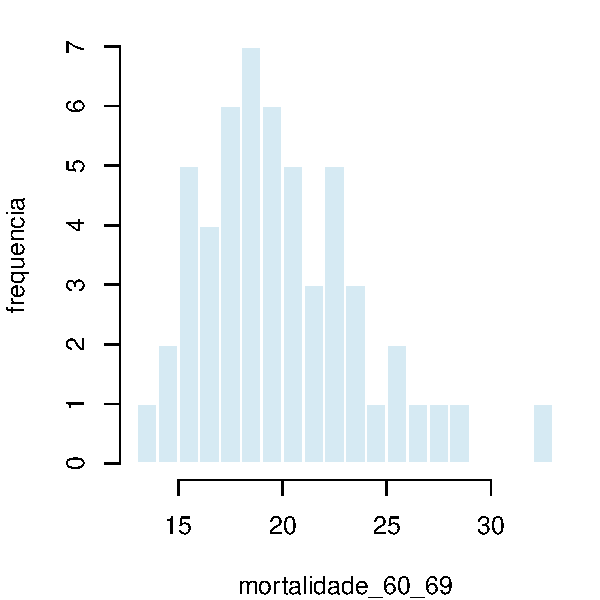
\includegraphics[width=0.52\linewidth]{figure/fig-resposta-1} 

}


\end{knitrout}
  \fonte{Elaborada pelos autores.}
\end{figure}

\textbf{Veredito.} Feche dizendo se a pergunta se sustenta.

A pergunta é \textbf{provisória}: será revista depois da Aula 12.

\postextual
\bibliography{referencias}

\end{document}
